\documentclass[UTF8,a4paper,11pt,fontset=none]{ctexart}
\usepackage{fontspec}\setmainfont{Times New Roman}\setsansfont{Arial}\setmonofont{Menlo}\setCJKmainfont{Songti SC}\setCJKsansfont{Heiti SC}
\usepackage[margin=2.1cm]{geometry}\usepackage{amsmath,amssymb,graphicx,booktabs,tabularx,hyperref,microtype}
\hypersetup{hidelinks}\setlength{\parskip}{.35em}\setlength{\emergencystretch}{2em}
\title{接收电流空间何时值得改变？\\论文中文稿、完整推导与从零解读}\author{}\date{}
% Use cached readable math sizes; no network font installation.
\DeclareMathSizes{10}{10}{7}{6}
\DeclareMathSizes{9}{9}{6}{6}
\DeclareMathSizes{8}{8}{6}{6}
\DeclareMathSizes{7}{7}{6}{6}
\DeclareMathSizes{6}{6}{6}{6}
\DeclareMathSizes{5}{6}{6}{6}
\begin{document}\maketitle
\section*{摘要：这篇论文研究什么}
接收器可以告诉我们哪些电流容易被观测，却不能直接告诉我们：由这些电流构成的模型会产生怎样的材料更新。本文从Maxwell方程出发，把一次指定电流改动拆成材料注入（material injection）、保留空间多重散射反馈（retained multiple-scattering feedback）和接收返回（receiver return），再追踪它怎样改变Gauss--Newton（GN）材料步。两组材料方向包含完整步差，但步差是否有用，还取决于曲率变化和当前残差的共同作用。

因此，我从接收基底出发，在固定电流维数下测试少量一列移出、一列移入的条件交换（conditional exchange）。更丰富的约化模型先排序，每轮最多两个候选接受完整定向切向作用$Jd$的数值复核；只有共同完整二次目标确实下降，才改变空间。接受阈值只使用在线数值尺度，不读取完整最优材料步或真值。原四对象的对象汇总完整GN gap中位下降65.2\%；冻结规则后，十个完整额外对象全部改善，中位下降50.7\%。另一个对象保留晚期前置求解失败。这里的gap衡量材料步对完整GN步的保真度，不是最终图像误差。暗电流、信息正而收益负、以及单方向负而联合方向正的物理见证，共同说明接收强度和信息汇总不足以决定当前材料用途。论文给出的结果是一个有明确费用和适用范围的电磁机制与条件设计。

\section*{怎样阅读这份材料}
这份材料同时提供论文的中文理解稿和入门解释。先建立材料、场、电流、测量之间的关系，再推导指定电流改变怎样影响材料步，最后说明每类实验回答哪个问题。所有主要推导用中文写出；读者不需要先读英文，也不需要了解内部项目编号。

只记住一个问题即可：已经有一个按接收器选出的可靠电流空间，什么时候值得换掉其中一个方向？本文不要求发明新的完整求解器。它把某次替换的物理影响算清楚，然后检查这个影响是否改善当前材料更新。
\setcounter{tocdepth}{1}\tableofcontents\clearpage
\section*{中英文术语与符号速查}\addcontentsline{toc}{section}{中英文术语与符号速查}
\markboth{中英文术语与符号速查}{中英文术语与符号速查}
\noindent\begin{tabularx}{\linewidth}{p{.23\linewidth}p{.31\linewidth}X}\toprule
中文名称&英文术语&用途\\\midrule
电磁逆散射&electromagnetic inverse scattering&从散射场估计材料。\\
感应电流&induced current&材料受总场激发产生的响应。\\
材料切向&material tangent&允许的微小材料变化方向。\\
材料注入&material injection&把材料变化变成电流方程右端。\\
保留空间反馈&retained feedback&新增方向激发已有电流后返回的响应。\\
反馈修饰&feedback-dressed&原方向加上保持保留方程一致的反馈。\\
材料拉回&material pullback&由伴随将输出影响返回材料变量。\\
双侧支撑&paired material support&两组材料方向包含指定模型改变的步差。\\
接收基底&receiver-derived basis&按直接接收谱建立的初始空间，仍需通过端点求解检查。\\
条件交换&conditional exchange&在当前已选空间下重算的一列替换。\\
较丰富约化参考&richer reduced anchor&用于排序的较大约化模型，不是完整最优解。\\
有限有符号收益&finite signed gain&实际位移在共同完整二次目标上减少的量。\\
高精度定向复核&high-fidelity directional check&计算$Jd$检查收益的数值方法。\\
数值显著性&numerical significance&收益超过预先固定的浮点尺度容差。\\
GN二次差距&full-GN quadratic gap&约化材料步相对完整最优步的局部误差。\\
候选覆盖&candidate coverage&短池实际包含多少可用机会。\\
弃权／无动作&abstention / no-op&没有接受的候选时保持当前空间。\\
线搜索&line search&在共同非线性目标上缩短并接受可行步。\\
\bottomrule\end{tabularx}

\begin{table}[htbp]\centering\small
\begin{tabularx}{\linewidth}{lX}\toprule
符号&含义\\\midrule
$\chi,Q_T,s$&材料对比度、物理正交展开、实材料更新。\\
$L,G_D,S,B,J$&内部方程、内部传播、接收、材料注入、材料导数。\\
$V,A,C,k$&交换公式中的共同核心、移出方向、移入方向、共享复电流列数。消元公式另以$A=I-L$表示内部传播，依公式上下文区分。\\
$\bar C,Y_C,N_C,\Gamma_C$&反馈修饰电流、观测因子、注入因子、Schur补。\\
$r,\Lambda,\ell,H,h$&数据残差、正则曲率、先验线性项、法方程矩阵和正号常数项。\\
$x,d,u,z,Q$&原材料步、实际步差、$r+J_Fx$、$J_Fd$、完整收益。\\
$s_*,R_{\rm GN},\rho_{\rm obj}$&离线完整参考步、完整GN差距、对象内求和风险比。\\
\bottomrule\end{tabularx}
\caption{电流列数与实材料维数是不同预算；复输出对应同一个共享实材料变量。}
\end{table}\clearpage


\section{背景：为什么电流子空间与材料更新之间还有一个问题}
电磁逆散射（electromagnetic inverse scattering，EIS）先用已知照明照射物体，再根据接收的散射场估计材料。正问题（forward problem）是材料已知时预测场；逆问题（inverse problem）是场已知时寻找材料。内部总场（total field）与感应电流（induced current）互相作用：材料响应产生电流，电流产生内部场，内部场又产生电流。

三维矢量Maxwell离散偶极子近似（discrete-dipole approximation, DDA）把物体离散成极化单元，每个单元保留三个场分量及并矢Green耦合（dyadic Green coupling，即三个分量之间的张量耦合）。离散方程解得精确，说明这个网格上的线性系统求解准确；与球体散射的独立Mie级数参考接近，才是在指定球体条件下检验连续散射。两者回答不同的问题。

子空间优化方法（subspace-based optimization method, SOM）利用接收Green算子的奇异结构辨认容易观测的电流。双重子空间优化方法（Twofold SOM, TSOM）进一步引入内部传播子空间；FFT-TSOM利用快速Fourier变换（fast Fourier transform, FFT）组织计算。这些方法已经考虑电流与材料的一致性以及内部作用。本文补上一个具体接口：改动一个既有电流子空间（current subspace）后，当前材料更新（material update）究竟怎样改变？

\begin{figure}[htbp]\centering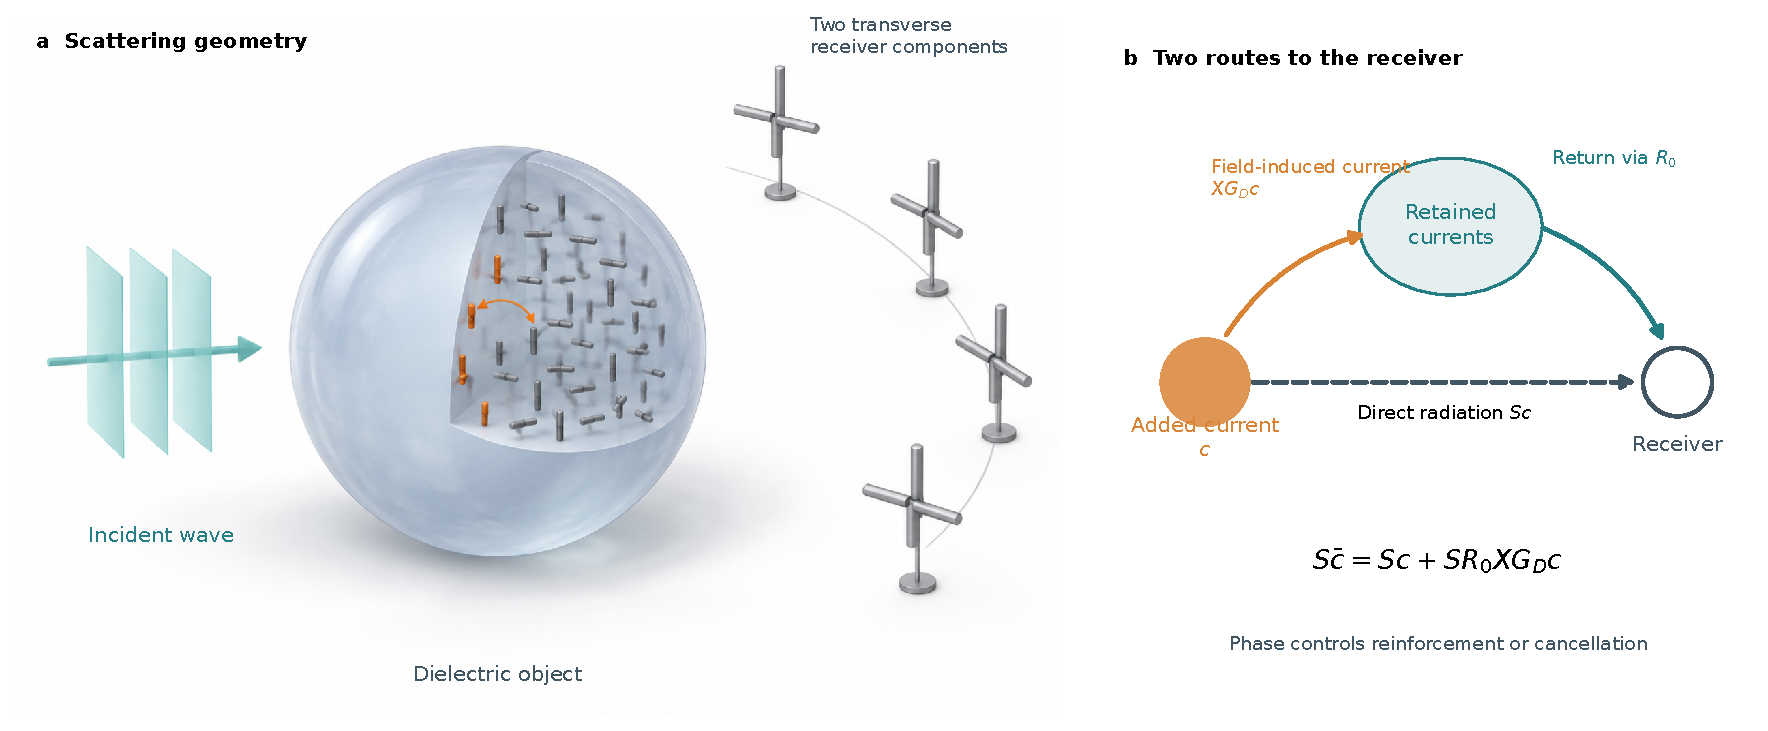
\includegraphics[width=.96\linewidth]{figures/physical_feedback.pdf}
\caption{材料、内部电流与接收的概念示意。新增电流有直接辐射和保留空间反馈两条返回路径；图中光线和局部电流是示意，不是计算场分布。}
\end{figure}

\section{从零读懂三条公式}
\subsection{材料扰动怎样到达接收器}
\[
J=SL^{-1}B.
\]
从右往左读：材料变化$s$通过真实注入（material injection）$Bs$形成电流激励；$L^{-1}$求全部多重散射（multiple scattering）后的电流变化；$S$计算接收响应。材料切向必须在体积加权的物理度量下正交化，复介电材料的实部和虚部是共享实变量。这样比较方向不会依赖人为参数单位。

\subsection{新增方向为什么不是只多一条直接辐射}
\[
\bar C=(I-R_0L)C=C+R_0XG_DC.
\]
这里$C$是新增电流方向，$R_0$是保留电流空间的求解算子，$X$是材料响应算子，$G_D$将电流变成内部场。右边第一项是新增方向本身，第二项是它激发保留电流后返回的响应。反馈（feedback）来自频域方程的消元。新增电流在内部产生场，保留电流对该场响应；二者的复振幅叠加后才到接收器。

\subsection{为什么完整材料步还要看残差}
\[
H_Us_U=-h_U,\qquad H_U=J_U^TJ_U+\Lambda,\quad h_U=J_U^Tr+\ell.
\]
曲率（curvature）描述材料方向的尺度和耦合；残差拉回（residual pullback）描述当前数据要求往哪个方向改；正则项（regularization）和线性prior项也参与。两个模型有相同$J^TJ$，仍可能有相反$J^Tr$。因此“模式信息强”还不足以决定它是否帮助当前材料步。

\section{如何读后面的实验}
完整GN差距是约化模型步相对同一完整模型最优步的二次误差。材料真值误差是估计材料与真实物体的物理距离。前者可以下降，后者仍可能上升，因为线性化、约束和步长尚需处理。

同一物体的三个状态、三个电流预算不是九个独立对象；同一计算五次计时也不是五份新物理证据。后面的表先按对象求和，再比较风险比；计时则单独衡量波动。读图时同时看绝对差距和相对比值，避免把越来越小的receiver分母误读为方法自身必然发散。

\clearpage\part{中文论文：从材料激发到实际更新}
\section{论文的数学设置：从材料到测量}
前面的部分给出了背景和直觉。下面按论文的论证顺序展开中文推导：先固定材料和测量的含义，再消去电流坐标，随后推导材料步变化与实际收益。这里整理的是英文正文和理论说明中已有的结果，不增加实验或改变成立条件。

\subsection{物理材料空间与多照明}
用 $\chi$ 表示介电对比度（dielectric contrast），$X$ 表示对应的材料响应算子（material-response operator）。第 $p$ 次照明的感应电流（induced current）满足
\begin{equation}
 j_p=X(e_p^{\rm inc}+G_Dj_p),\qquad L=I-XG_D.
\end{equation}
$G_D$ 是内部矢量 Green 算子（internal vector Green operator），$e_p^{\rm tot}=e_p^{\rm inc}+G_Dj_p$ 是总场（total field）。材料变化用实坐标 $s\in\mathbb R^d$ 表示；复介电材料的实部和虚部都是这个实向量的组成部分。物理材料切向（physical material tangent）$Q_T$ 满足
\begin{equation}
 \delta\chi=Q_Ts,\qquad Q_T^\top M_\chi Q_T=I.
\end{equation}
这里的等式在实化坐标中理解，$M_\chi$ 是体积加权的材料 $L^2$ 内积。这样，同一材料子空间仅仅换单位或旋转坐标，不会人为改变某个方向的重要性。

对电流方程求方向导数（directional derivative），得到
\begin{equation}
 L\,\delta j_p=DX[Q_Ts]e_p^{\rm tot}=:B_ps,
 \qquad K_p=L^{-1}B_p,\qquad J_p=SK_p.
\end{equation}
$B_p$ 是材料注入映射（material-injection map）：它将材料扰动转成电流方程的右端。实际电流变化是 $K_ps$，并不是 $B_ps$。$S$ 包括接收、归一化与需要时的噪声白化（noise whitening）；$J_p$ 是材料到测量的 Jacobian。

所有照明共享同一个材料向量 $s$，但有各自的电流。把各次测量的实部、虚部纵向堆叠（stacking），形成实线性映射 $J$。后面的 $J^*$ 是该实材料内积下的伴随（adjoint）。例如，复输出矩阵 $F$ 作用于实材料坐标时，伴随为 $v\mapsto\operatorname{Re}(F^Hv)$，不能遗漏取实部。电流分块公式可先用复记号写出，再对照明做块对角提升和实化（realification）。

\subsection{DDA 中极化率的导数必须保留}
实际离散偶极子近似（discrete-dipole approximation, DDA）使用极化率（polarizability）$a(\chi)$，而不是把 $X$ 直接替换为 $\chi$。对体积为 $v$ 的单元，所用模型为
\begin{equation}
 a(\chi)=\frac{3v\chi}{\chi+3-i3c_kv\chi},\qquad
 a'(\chi)=\frac{9v}{(\chi+3-i3c_kv\chi)^2},\qquad c_k=\frac{k^3}{6\pi}.
\end{equation}
在偶极矩坐标下，$L=I-D_aG_{\rm off}$，扰动激励包含 $a'(\chi)\delta\chi\,e_p^{\rm tot}$；电流范数再按单元体积归一化。因而材料注入同时依赖当前材料、局部总场和允许的材料方向。把 $a$ 当成对比度，或者漏掉 $a'$，都会改变实际研究的材料导数。完整离散Green核及坐标因子见英文补充材料第1节。

\subsection{冻结状态下的局部材料问题}
固定当前材料、照明、残差和正则化。令 $r$ 为预测减观测的测量残差（data residual），$\Lambda\succ0$ 为正则化及阻尼曲率，$\ell$ 为共同的先验线性项。Gauss--Newton局部二次模型写成
\begin{equation}
 \begin{aligned}
 \Phi(s)&=\tfrac12\|r+Js\|^2
             +\tfrac12s^*\Lambda s+\ell^*s\\
 &=\tfrac12s^*Hs+h^*s+\tfrac12\|r\|^2,\qquad
 H=J^*J+\Lambda,\quad h=J^*r+\ell.
 \end{aligned}
\end{equation}
这里 $H$ 是正则化 Gauss--Newton Hessian，也就是材料法方程（material normal equation）的矩阵，不是包含全部二阶导数的精确非线性 Hessian。完整局部解为 $s_*=-H^{-1}h$，并且
\begin{equation}
 \Phi(s)-\Phi(s_*)=\tfrac12\|s-s_*\|_H^2,
 \qquad \|u\|_H^2=u^*Hu.
\end{equation}
因此，局部二次误差和 $H$-范数步误差等价；它们都不等于最终材料重建误差。

\section{消去保留电流：反馈修饰的导数变化}
\subsection{从分块电流方程得到 Schur complement}
设 $V$ 为原先保留的正交电流基，$C$ 为指定新增候选基（candidate bank），满足 $V^*V=C^*C=I$、$V^*C=0$。令 $A=I-L$，并用 $A_{VC}=V^*AC$ 等记号表示分块。假设 $D_V=I-A_{VV}=V^*LV$ 可逆，原电流响应为
\begin{equation}
 R_0=VD_V^{-1}V^*,\quad K_0=R_0B,\quad J_0=SK_0.
\end{equation}
注意 $R_0$ 作用在电流空间；后面 $M_0=(J_0^*J_0+\Lambda)^{-1}$ 作用在材料空间。

对任意材料右端，增广后的电流写成 $V\alpha+C\gamma$。Galerkin投影要求方程残差与整个保留空间正交，因此
\begin{equation}
 \begin{bmatrix}D_V&-A_{VC}\\-A_{CV}&I-A_{CC}\end{bmatrix}
 \begin{bmatrix}\alpha\\\gamma\end{bmatrix}
 =\begin{bmatrix}B_Vs\\B_Cs\end{bmatrix},
 \qquad B_V=V^*B,\quad B_C=C^*B.
\end{equation}
第一行给出 $\alpha=D_V^{-1}(B_Vs+A_{VC}\gamma)$。代入第二行后，新增坐标满足
\begin{equation}
 \Gamma_C\gamma=N_Cs,
 \quad\Gamma_C=I-A_{CC}-A_{CV}D_V^{-1}A_{VC},
 \quad N_C=B_C+A_{CV}D_V^{-1}B_V.
\end{equation}
$\Gamma_C$ 是 Schur补矩阵（Schur complement），描述新增空间自身作用和新增—保留—新增反馈回路。$N_C$ 则是消去原坐标后，材料真正进入新增方程的激励。

\subsection{反馈修饰切向分解及其物理含义}
定义
\begin{equation}
 \bar C=C+VD_V^{-1}A_{VC}=(I-R_0L)C,\qquad Y_C=S\bar C.
\end{equation}
只要 $\Gamma_C$ 可逆，回代立即得到
\begin{equation}\label{zh:tangent}
 \boxed{K_C-K_0=\bar C\Gamma_C^{-1}N_C,\qquad
 J_C-J_0=Y_C\Gamma_C^{-1}N_C.}
\end{equation}
这就是反馈修饰切向分解（feedback-dressed tangent factorization）。在对比源表述下，$A=XG_D$，于是
\begin{equation}
 \bar C=C+R_0XG_DC,\qquad Y_C=SC+SR_0XG_DC.
\end{equation}
$SC$ 是直接辐射；$G_DC$ 是新增电流产生的内部场；$XG_DC$ 是该场激发的材料电流作用；$R_0$ 进一步处理保留空间中的相互散射。接收器看到两条路径的复振幅叠加，既可能增强，也可能抵消。另一侧 $N_C=B_C+A_{CV}D_V^{-1}B_V$ 表明，材料既能直接激发新增方向，也能先激发保留方向再传到新增方向。

这不是给直接输出乘一个经验增益。一般 $\bar C$ 不再与 $V$ 欧氏正交，却满足 $V^*L\bar C=0$：它正是保持原Galerkin方程不被破坏的修正。整个解释是频域反馈（frequency-domain feedback），不额外假定控制系统的时域稳定性。

\subsection{弱反馈的绝对界与相对界不同}
若 $\|A_{VV}\|_2\le\eta<1$，Neumann级数给出 $\|D_V^{-1}\|_2\le(1-\eta)^{-1}$，从而
\begin{equation}
 \|Y_C-SC\|_2\le\frac{\|SV\|_2\|A_{VC}\|_2}{1-\eta}.
\end{equation}
要相对直接输出给出统一保证，还需要 $SC$ 在所研究系数空间中有正的最小奇异值：
\begin{equation}
 \frac{\|(Y_C-SC)u\|_2}{\|SCu\|_2}
 \le\frac{\|SV\|_2\|A_{VC}\|_2}
 {(1-\eta)\sigma_{\min}(SC)},\qquad u\ne0.
\end{equation}
对于严格位于接收零空间的电流（receiver-dark current），这个正下界不存在；近乎暗的方向即使有很小的正奇异值，相对界也可能大到无法提供有用保证。它的绝对反馈可以不大，却远大于直接输出。因此，大的反馈/直接比值本身不能证明谐振；高材料对比度也不能单独证明反馈一定强。

\section{材料步为什么需要两组方向：闭包定理的中文证明}
令 $T_C=\Gamma_C^{-1}N_C$，于是 $J_C=J_0+Y_CT_C$。在相同 $r,\Lambda,\ell$ 下，定义
\begin{equation}
 \begin{aligned}
 H_0&=J_0^*J_0+\Lambda,& M_0&=H_0^{-1},\\
 s_0&=-M_0(J_0^*r+\ell),&
 s_C&=-(J_C^*J_C+\Lambda)^{-1}(J_C^*r+\ell).
 \end{aligned}
\end{equation}
\paragraph{定理：双侧材料步闭包（paired material-step closure）。}
这里的观测、Schur和注入因子需要一起实化。$P$为照明次数；先对照明作块对角提升 $\mathbf Y=I_P\otimes Y_C$、$\Gamma_{\rm blk}=I_P\otimes\Gamma_C$，纵向堆叠注入 $\mathbf N$，再定义 $\mathcal R(F)=[\operatorname{Re}F,-\operatorname{Im}F;\operatorname{Im}F,\operatorname{Re}F]$ 和 $\widehat N=[\operatorname{Re}\mathbf N;\operatorname{Im}\mathbf N]$。于是 $\widehat D=\mathcal R(\mathbf Y)\mathcal R(\Gamma_{\rm blk})^{-1}\widehat N$，与数据的固定堆叠顺序只差一个排列。以下材料空间公式中的 $Y_C,\Gamma_C,N_C$ 指这组实化因子，伴随为实转置。这一步保留跨照明共享材料，不能把一个复电流方向误当作一个实材料秩。
在上述可逆性、共同正则化和精确算子作用条件下，若没有截掉非零作用方向，则
\begin{equation}\label{zh:closure}
 \begin{aligned}
 s_C-s_0={}&-M_0J_0^*Y_C(T_Cs_C)\\
 &-M_0N_C^*\Gamma_C^{-*}Y_C^*(r+J_Cs_C)
 \in\mathcal E_0(C),\\
 \mathcal E_0(C)&=\operatorname{Range}M_0[J_0^*Y_C,N_C^*].
 \end{aligned}
\end{equation}
\paragraph{证明。}
展开曲率差和线性项差：
\begin{equation}
 \begin{aligned}
 \Delta H&=J_0^*Y_CT_C+T_C^*Y_C^*J_0+T_C^*Y_C^*Y_CT_C,\\
 \Delta h&=T_C^*Y_C^*r.
 \end{aligned}
\end{equation}
两套法方程相减，得到
\begin{equation}
 H_0(s_C-s_0)=-\Delta Hs_C-\Delta h
 =-J_0^*Y_CT_Cs_C-T_C^*Y_C^*(r+J_Cs_C).
\end{equation}
左乘 $M_0$，再使用 $T_C^*=N_C^*\Gamma_C^{-*}$，即得式\eqref{zh:closure}。\hfill$\square$

第一组 $M_0J_0^*Y_C$ 是观测侧材料拉回（observation-side material pullback）：新增观测响应与原材料敏感度发生耦合，改变原有材料方向上的步长。第二组 $M_0N_C^*$ 是注入侧材料拉回（injection-side material pullback）：更新后的测量残差沿新增激励路径返回材料空间。只看右端改变 $\Delta h$ 会漏掉第一组中的曲率耦合。

闭包告诉我们步差可能出现在哪里，并不保证当前步一定改变。若 $r=0,\ell=0$，即使 $J_C-J_0\ne0$，仍有 $s_C=s_0=0$。物理通路给出影响的可能性，当前残差和正则化决定它是否实际参与更新。

\subsection{非单调曲率的最小例子}
取
\begin{equation}
 J_0=[1,0],\quad J_C=[1,1],\quad\Lambda=I,\quad r=1,\quad\ell=0.
\end{equation}
直接求解可得 $s_0=(-1/2,0)^\top$、$s_C=(-1/3,-1/3)^\top$，步差为 $(1/6,-1/3)^\top$。观测侧沿第一个材料坐标，注入侧沿第二个材料坐标，单独一侧都无法表达全部步差。同时
\begin{equation}
 \Delta H=\begin{bmatrix}0&1\\1&1\end{bmatrix},\qquad\det\Delta H=-1.
\end{equation}
因此曲率差是不定矩阵（indefinite matrix）。这个例子可嵌入 $L=I$ 的Galerkin模型，说明不定性不要求多重散射才能发生。Maxwell反馈决定实际物理因子；最小二乘法方程本身产生两侧耦合。增加电流空间是改进已有测量模型，不是增加独立测量，二者不能混为一谈。

\subsection{结构闭包与当前误差对齐是两件事}
设 $Z$ 是 $\mathcal E_0(C)$ 的独立基。在不改变完整局部目标的前提下，令修正步为 $s=s_0+Zq$。记完整目标在 $s_0$ 的梯度缺陷为 $d_0=Hs_0+h$，则
\begin{equation}
 q_*=-\bigl(Z^*HZ\bigr)^{-1}Z^*d_0,
 \qquad
 \Phi(s_0)-\Phi(s_0+Zq_*)
 =\tfrac12 d_0^*Z(Z^*HZ)^{-1}Z^*d_0.
\end{equation}
因为 $s_C$ 在这个仿射空间中，最优修正一定不差于指定的 $s_C$。但增益取决于 $Z^*d_0$；若它为零，修正没有收益。用 $P_Z$ 表示到 $H^{1/2}Z$ 的正交投影，还可把增益写为 $\tfrac12\|P_ZH^{-1/2}d_0\|^2$。这解释了为什么完整描述某个模型变化的方向，不一定是消除当前完整误差的最佳方向。材料Krylov方向直接从误差出发，完全可能更有效。

\section{从电流模型改变到材料信息、残差方向和实际收益}
\subsection{为什么要从一个可靠的接收基底出发}
接收谱基底（receiver spectral backbone）按电流直接产生的接收响应保留方向。它的好处是定义清楚、容易复现，而且已有比较显示它在较大的电流预算下相当可靠。现在的问题不是从空集重新寻找所有方向，而是保留这一基础，只检查少量替换是否值得。

一次替换有两个端点：原空间 $[V,A]$ 和新空间 $[V,C]$。$V$ 是共同保留的电流核心（common retained core）；$A$ 是移出的方向，$C$ 是移入的方向。两端使用相同材料状态、照明、正则化和测量残差。若共同核心和相应Schur块可逆，前面的反馈分解给出
\[
 D=J_n-J_o=Y_C\Gamma_C^{-1}N_C-Y_A\Gamma_A^{-1}N_A.
\]
两个项都包含材料激发、内部反馈和接收返回，因而替换后的影响不是两个裸接收强度的差。如果共同核心不可逆，但两个端点本身稳定，就直接计算端点；不能把快速公式不能用，误写成物理空间不可行。

\subsection{材料信息描述响应，残差拉回描述当前任务}
在共同的实材料坐标中，定义数据曲率（data curvature）
\[
 \mathsf I_U=J_U^TJ_U.
\]
给一个材料变化 $v$，$v^T\mathsf I_Uv=\|J_Uv\|^2$，描述模型认为这种变化会产生多强的接收响应。这里的 $\mathsf I_U$ 表示数据曲率，不是独立测量数量，也不包含当前残差方向。

材料步还需要常数梯度项（constant gradient term）
\[
 h_U=J_U^Tr+\ell,\qquad H_Us_U=-h_U.
\]
它保留接收响应与当前残差的方向、符号和复相位的实拉回。保存的数据把这个正号量写成 $b$；真正的法方程右端是 $-h_U$，不是 $h_U$。

令 $D=J_n-J_o$。直接展开两端点，可得
\[
 \Delta\mathsf I=J_o^TD+D^TJ_o+D^TD,
 \qquad \Delta h=D^Tr.
\]
再从 $H_ns_n=-h_n$ 减去旧端点的关系：
\[
 H_n(s_n-s_o)=-(h_n-h_o)-(H_n-H_o)s_o.
\]
由于正则项共同不变，$H_n-H_o=\Delta\mathsf I$，因此
\[
 \boxed{d=s_n-s_o=-H_n^{-1}(\Delta h+\Delta\mathsf I s_o).}
\]
这几行是从物理导数变化到实际更新的完整桥梁。只给出信息谱，会丢掉 $\Delta h$；只讨论残差右端，又会丢掉曲率改变。

一个简单代数例子能说明这一点。取 $r=1$、$\ell=0$、$\Lambda=1$。$J=1$ 与 $J=-1$ 的信息曲率都是1，却分别给出 $s=-1/2$ 与 $s=1/2$。它们有相同的信息量汇总，更新方向完全相反。这个例子是解释公式，不是新增电磁数据。

\subsection{信息增加和模型更准确要分别衡量}
近似模型可能过度放大某些材料响应，因此更大的信息体积不一定更接近完整物理。本文使用固定尺度 $P_0$，报告有效维数（effective dimension）与信息体积诊断（information-volume diagnostic）：
\[
 d_{\rm eff}=\sum_i\frac{\nu_i}{1+\nu_i},\qquad
 \mathcal D=\frac12\sum_i\log(1+\nu_i),
\]
其中 $\nu_i$ 是 $P_0^{-1/2}\mathsf I_UP_0^{-1/2}$ 的特征值。同时报告相对完整参考的信息保真度（information fidelity），而不是只奖励 $\mathcal D$ 变大。

实际比较把 $P_0=10^{-5}I$ 的先验尺度与Levenberg--Marquardt阻尼（LM damping）分开；局部求解仍使用原有总曲率。接收数据沿用固定数值归一化，尚无独立标定的噪声协方差，所以这些量作为尺度归一化曲率诊断，不宣称为硬件测量的互信息。较小的Gaussian材料空间可以算完整谱；voxel空间只在共同的16个材料方向上诊断，不能据此说完整空间没有弱方向。

\subsection{实际位移在完整二次目标上是否值得}
生成 $d$ 以后，用同一个完整冻结二次目标评价有符号收益（finite signed gain）：
\[
 Q=\Phi_F(x)-\Phi_F(x+d)=-g_F(x)^Td-\tfrac12d^TH_Fd.
\]
第一项检查位移是否朝向下降，第二项扣除这段有限位移的曲率代价。$Q>0$表示更忠实于当前完整GN更新；它没有把材料真值加入目标，所以不能直接保证图像更准确。

为检查这个标量，不必再计算一次完整伴随（full adjoint）。先缓存 $u=r+J_Fx$，对候选只算定向输出（directional output）$z=J_Fd$：
\[
 Q=-u^Tz-(\ell+\Lambda x)^Td
     -\tfrac12(\|z\|^2+d^T\Lambda d).
\]
复表示下第一项取 $\operatorname{Re}\langle u,z\rangle$。每个材料方向仍要支付所有照明的全波右端；这只是减少不必要的伴随计算，并不意味着免费。接受后更新空间、材料步及缓存输出，下一轮重算条件评分（conditional scoring）。

\subsection{高精度复核与严格证书的区别}
如果输出有经过验证的误差界 $e_u,e_z$，则收益误差可由
\[
 \epsilon_Q=e_u\|\widehat z\|+(\|\widehat u\|+\|\widehat z\|)e_z+e_ue_z+\tfrac12e_z^2
\]
控制。接受一个动作需要其收益下界为正；证明整个声明邻域没有好动作，需要每个可行动作的收益上界都低于容差。这是两个不同判断。

现有全波输出尚无这样闭合的严格界，所以实验采用双精度定向复核（high-fidelity directional check），不把数值容差当作确定性证书（deterministic certificate）。若只检查少量候选，没有找到好动作，就保留未解决状态；三次动作预算用完也不是局部最优的证明。

\subsection{怎样阅读方向分解图}
信息方向固定为同一个完整参考的特征子空间，而不是每换一个模型就重新给特征向量编号。Gaussian空间中，总求解曲率在这些方向上的权重是数据曲率加先验和LM项，因此各带的步误差能量可以精确相加；参考步尚有微小梯度时，另保留其线性交叉项。

一个约化模型认为很弱的方向，可能只是它没有表示出来；完整模型仍可能对此很敏感。这叫约化模型假弱（ROM-false-weak），与真实数据弱（true data-weak）不同。成功交换可能修复假弱、减少过度曲率或调整残差方向，并不必然是在给真实弱方向补先验。

\section{从机制变成具体决定：接收基底上的条件交换}
\subsection{保留可靠的起点，只检查指定替换}
接收基底（receiver-derived basis）是接收算子中直接辐射最强的前$k$个奇异方向。本文从这个可复现的空间出发，问一个更具体的问题：移出一个已有方向、移入一个候选方向，生成的材料步是否更忠实于完整模型？被保留的是电流总维数，原接收方向可以被替换。所有照明共享$k=4,8,16$列复电流；材料变量、总场、完整前向残差、正则项和阻尼保持不变。接收起点仍须通过预设的端点稳定性与法方程残差检查，接收谱本身不保证内部求解一定稳定。

程序先获得固定字典中的电流候选。候选来自六类信息：接收模式（receiver modes）、内部传播（internal propagation）、Fourier模式、anchor的正向/伴随响应（primal/dual responses）、anchor电流方程的剩余激励（current residual）以及固定随机电流。按这个顺序循环，从每类取两个尚未选中的方向，构成12个移入方向的短候选池（incoming short pool）。一个64列的较丰富约化参考（richer reduced anchor）用于排序。Anchor不是完整最优解，也不含真值；获取它的物理作用和时间单独收费。缓存投影矩阵所用的辅助空间只是计算载体，不代表实际保留秩；每个端点仍严格为$k$列。

移出一个方向以后，剩下共同电流核心（common current core）。对每个可行移入方向，求解新端点模型，用真实端点步差$d$在anchor目标上排序。每轮最多两个候选进入完整定向复核（full directional verification），计算$J_Fd$并评价$Q$。只有超过在线数值阈值的候选才接受；否则保持当前空间，即无动作（no-op）。接受以后重新计算共同核心、耦合和评分，最多接受三次。

没有测试到好候选，只能说明这个短池和这次复核没有找到可接受动作；池外可能还有好方向。因此停止时使用未解决弃权（abstention），不说已达到整个字典的局部最优。两列联合见证解释了动作之间的条件依赖，但本文没有因此改变冻结的一列交换规则。

\subsection{在线数值阈值：不需要完整最优材料步}
方向公式中每项可能发生相消。程序先累计它们的绝对量，再加入当前输出和基点的量级，构成数值尺度（numerical scale）：
\begin{align*}
S_Q={}&\sum_i|u_i||z_i|+\sum_j|(\ell+\lambda x)_j||d_j|\\
&+\tfrac12\|z\|^2+\tfrac12\lambda\|d\|^2+\|r\|^2+\|u\|^2\\
&+|\ell^Tx|+\lambda\|x\|^2.
\end{align*}
这里实现的$\Lambda=\lambda I$；$u=r+J_Fx$是执行这一步后的线性化残差，$z=J_Fd$是候选位移的测量变化。令$m_R$为测量实化后的维数、$d_R$为材料实维数，$n=m_R+3d_R+16$。使用FP64相对机器精度$\epsilon_{64}$，冻结阈值
\[
\tau_{\rm online}=32\,\mathrm{tiny}_{64}
+32\frac{n\epsilon_{64}}{1-n\epsilon_{64}}S_Q.
\]
其中$\mathrm{tiny}_{64}$是实现采用的FP64最小正正规数（smallest positive normal number），不是可调阈值。常数32和尺度表达式在验证结果出现前固定；判断为$Q>\tau_{\rm online}$。完整最优步$s_*$、真值和评估底噪不进入该阈值。原36个单元的真实物理回放表明，75个接受动作、每一步材料向量和输出以及最终风险全部保持相同。

这个阈值控制数值显著性（numerical significance），没有证明DDA离散误差或完整输出误差的严格半径。因此称高精度数值复核（high-fidelity numerical verification），不称确定性认证（deterministic certification）。较小的求解残差说明离散线性方程被解得准确，不能独自给出连续Maxwell输出的误差界。

\subsection{三个不同层次的结果}
冻结更新保真度（frozen-update fidelity）用$R_{\rm GN}$判断约化材料步离完整GN步有多远。含噪检验（noise validation）改变同一物理状态的残差，每份残差有自己的完整GN参考。非线性迁移（nonlinear transfer）则从相同初始化真正迭代材料，使用可行性投影（feasibility projection）和线搜索（line search），比较最终材料与真值。前一层改善不能代替后一层结果。

独立统计单位是对象（object），不是该对象的状态、预算或噪声次数。先把对象内的绝对GN差距相加，再计算相对receiver的比值；同时保留绝对差距和$H$范数步误差。这样，不会把高$k$时极小的receiver分母误读为普遍改善或普遍退化。

\clearpage\part{中文论文：物理见证、冻结验证与迁移}
\section{四个物理见证：从可以影响，到值得改变}
\subsection{直接看不见的电流，能通过保留空间返回}
在受控的$5^3,6^3,7^3$三维矢量Maxwell网格上，构造直接输出落入接收数值零空间的两列电流。$\|SC\|$低于$1.7\times10^{-16}$，但反馈后的$\|S\bar C\|$分别为0.0672、0.0720、0.0888，指定增广带来的材料导数变化为3.56\%、3.98\%、5.22\%。新增方向本身几乎不辐射到接收器，但它激发保留电流，后者辐射到接收器。这就是接收暗电流（receiver-dark current）仍可改变材料导数的明确路径。

\begin{figure}[htbp]\centering\includegraphics[width=.9\linewidth]{figures/path_depth_dark.pdf}
\caption{直接输出和反馈后输出是不同对象。这个图检验受控物理通路，并不证明所有暗电流值得保留。}
\end{figure}

\subsection{信息更多，实际步仍可能更差}
信息体积（information volume）和有效维数（effective dimension）是材料响应谱的两个汇总量。固定正尺度$P_0$，设$\nu_i$为$P_0^{-1/2}J_U^TJ_UP_0^{-1/2}$的特征值，定义
\[
\mathcal D(U)=\tfrac12\sum_i\log(1+\nu_i),\qquad
d_{\rm eff}(U)=\sum_i\frac{\nu_i}{1+\nu_i}.
\]
它们回答模型在这个尺度下有多少、多强的材料响应。这里用$P_0=10^{-5}I$；没有实测噪声协方差标定，因此不把数值直接当成硬件互信息。信息保真度（information fidelity）另问这个曲率离完整模型有多远。这里的离线指标为$e_I(U)=\|(\mathsf I_F+P_0)^{-1/2}(\mathsf I_U-\mathsf I_F)(\mathsf I_F+P_0)^{-1/2}\|_2$，其中$\mathsf I_U=J_U^TJ_U$、$\mathsf I_F=J_F^TJ_F$；它衡量相对完整曲率的归一化误差，越小越接近。

一个近接触Maxwell对象的$k=4$替换得到$\Delta\mathcal D=6.3127$、$\Delta d_{\rm eff}=1.8613$，某个曲率保真度指标还略有改善，但完整收益$Q=-5.5754\times10^{-5}$。这一步反而更不忠实于完整GN目标。原因应从$\Delta h$与$\Delta\mathsf I s_o$的共同作用分析，不能仅凭这个见证说常数项单独导致失败。信息量描述响应；当前残差决定需要哪种响应。

\subsection{单独不利的方向，联合可能有利}
同一个rank14核心上，分别添加两列的收益为$Q_A=-3.2391\times10^{-8}$和$Q_B=-5.8389\times10^{-8}$，联合添加到rank16却得到$Q_{AB}=3.4787\times10^{-7}$。预先固定的540个pair测试中，有5个满足这种模式。配对相互作用（pair interaction）说明作用不一定可按单列相加；这些添加并非同秩交换，也不能据此推出所有Maxwell问题的普遍非次模定理。

\begin{figure}[htbp]\centering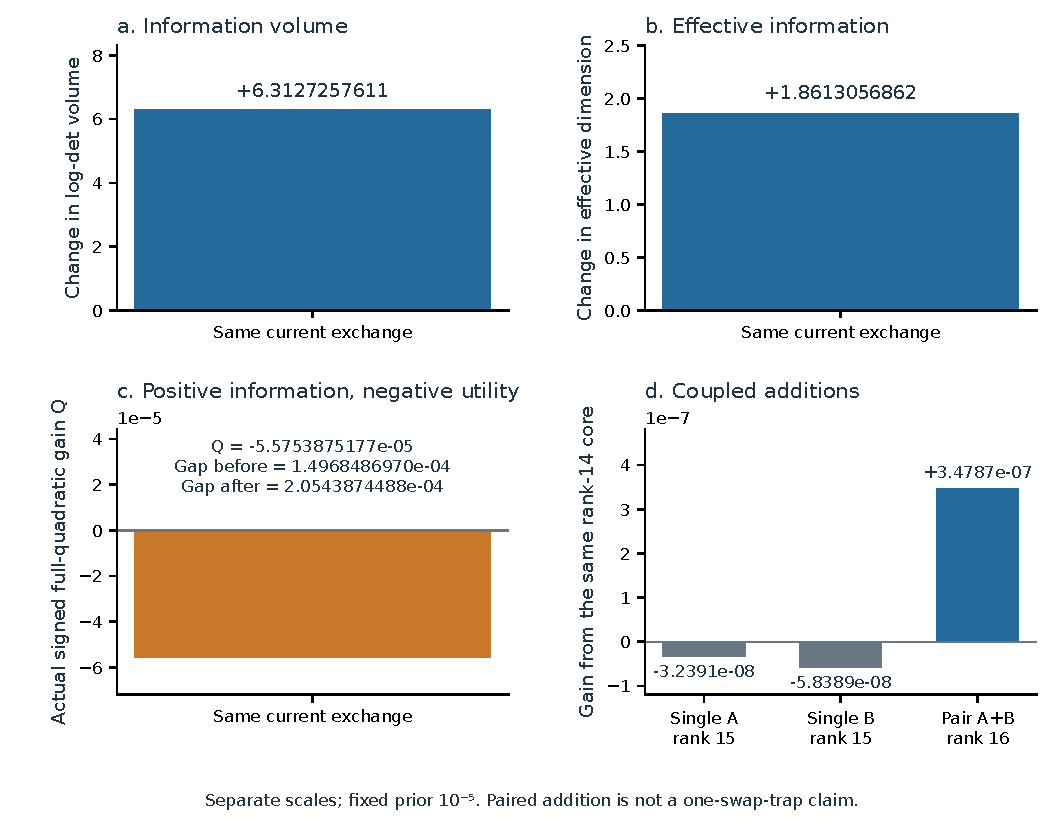
\includegraphics[width=\linewidth]{figures/information_and_pair_witness.pdf}
\caption{左侧说明信息体积及有效维数上升不足以判断实际收益，右侧展示同一核心的两单列与联合添加。各量使用自己的单位。}
\end{figure}

\subsection{必须评价真实位移的有限代价}
受控诊断使用同一批候选，分开位移构造和收益评价。$v$是旧曲率给出的一阶近似位移（first-order displacement），$d=s_n-s_o$是实际端点位移（actual endpoint displacement）；每种位移分别用线性项或完整二次式排序，最后统一执行真实$d$。

故意移除no-op、强制选择top-one时，$-g_F^Td$在29/36单元挑中负收益，加入$-\tfrac12d^TH_Fd$以后只有1/36。有限位移的曲率代价（finite-displacement curvature cost）确实改变候选排序。部署程序仍有no-op和真实$Jd$复核；上述计数是诊断结果，不是部署失败率。

\section{实验一：相同电流维数，比较完整材料步}
实验中的每个模型最终保留相同的$k=4,8,16$列复电流，所有照明共用这个空间。完整正问题、材料注入、残差、prior和LM阻尼一致；唯一改变的是电流空间里保留哪些方向。较大的anchor和dictionary只是取得候选的辅助信息，不算进最终电流秩，却必须计入费用。

使用三维矢量Maxwell DDA，计算域边长1.5，波数$k_0=2$；反演网格$12^3$、生成数据的网格$14^3$。六次平面波照明、64个双极化接收器。两张网格都来自同一DDA实现族，因此较细网格可以减轻正反问题使用完全相同离散模型造成的过于理想评估（inverse crime），但不等同于另一个独立全波求解器。材料方向使用体积加权正交Gaussian或voxel展开，极化率导数保留。

对每个对象，取初始化、保存迭代索引3及最后保存的状态，再比较三个电流预算。我们先在对象内部对所有绝对GN gap求和，然后计算
\[
\rho_{\rm obj}=\frac{\sum R_{\rm exchange}}{\sum R_{\rm receiver}}.
\]
小于1说明这种空间选择让该对象的材料步更接近完整GN步。它不意味着材料真值误差也减少相同比例。状态与预算是同一对象上的相关观测；对象才是统计汇总单位。

\subsection{原四对象：有明确收益，不能代替外部检验}
四对象分别为平滑Gaussian、近接触Gaussian、分层voxel、非对称voxel。36个单元中35个改善、1个相同，四个对象风险比分别为0.1904、0.6538、0.2776、0.4181，中位0.3478，即完整GN gap中位下降65.2\%。这些对象参与过方法形成，因此单靠它们不能证明推广效果。更换在线阈值后，36个单元的真实物理回放保持75次接受、全部终态空间和材料步逐位一致，说明部署定义修正没有改变这一结果。

\subsection{额外对象：规则锁定以后，十个完整对象都改善}
所有十一项兼容资产在看到交换结果前进入预先锁定的资产清单（manifest）。十个对象完整提供九个单元，均改善；中位风险比0.4928，下降50.7\%。四分位区间为[0.3314,0.5588]，按对象重采样（object bootstrap）得到的中位数95\%区间为[0.3133,0.5647]。另外一个非对称voxel对象完成六个早/中期单元，比值0.4925；晚期第一个预算的receiver端点没有通过预设法方程残差（normal-equation residual）检查，其余两个预算未运行。故覆盖是96/99，不能写成99/99成功。

\begin{figure}[htbp]\centering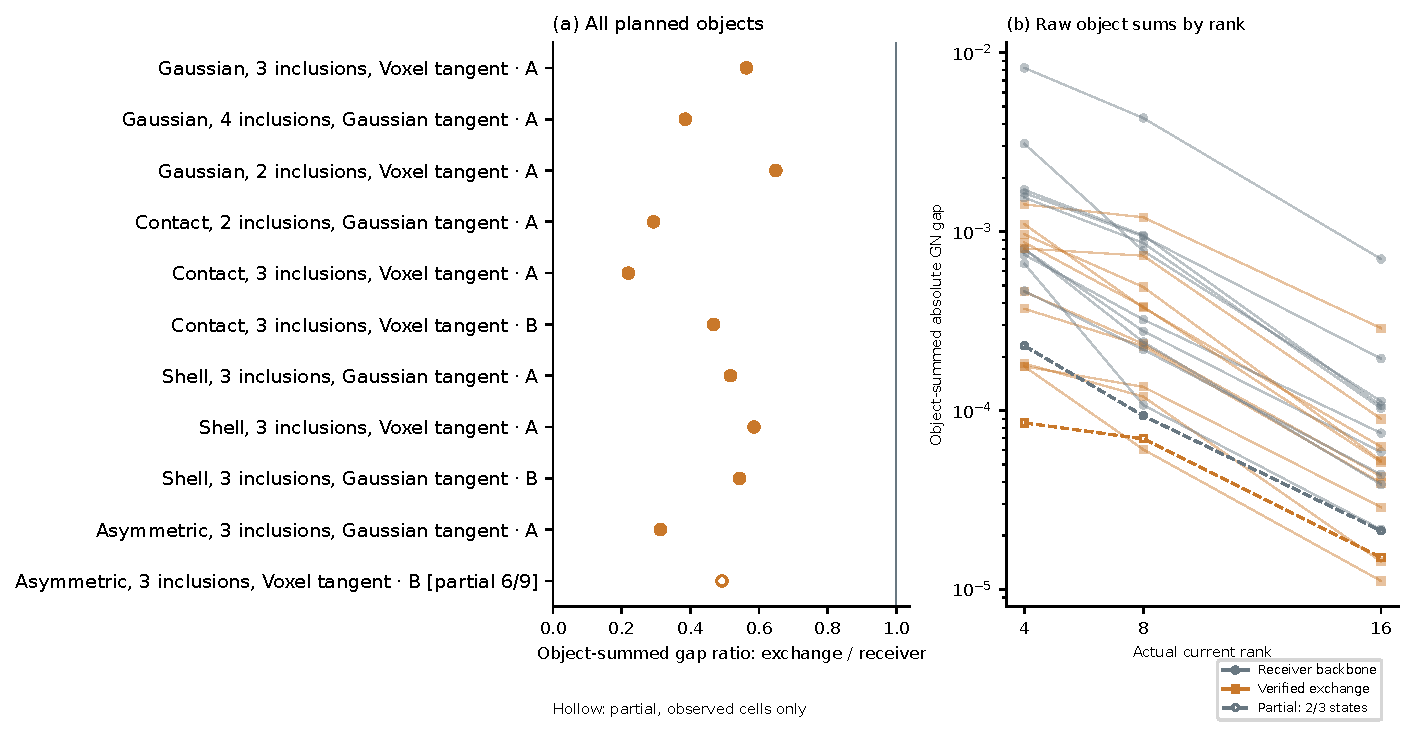
\includegraphics[width=.98\linewidth]{figures/closure_validation_v2/Figure1_primary_overview.pdf}
\caption{怎样读图：左图每个点对应一个对象的gap总和比值，1表示没有改善；空心点只有六个单元。右图把不同电流秩下的绝对gap同时画出，灰色为receiver，橙色为exchange；虚线表示该对象只有两个状态。较高电流秩通常使两种gap都变小，但仍需逐对象比较。}
\end{figure}

96个有效单元中95个改善、1个相同。receiver绝对gap范围为$2.74\times10^{-7}$至$3.09\times10^{-3}$，exchange为$8.73\times10^{-8}$至$8.36\times10^{-4}$。最小分母仍是对应evaluation floor的$6.31\times10^9$倍；最大完整参考真相对法方程残差为$9.55\times10^{-12}$。这说明下降不是参考底噪放大的假象。

这些资产曾用于宽域电流选择研究。没有找到它们用于历史交换的离线完整收益参考（exchange teacher）或试验网络（network pilot）的记录，但也不能保证历史结果完全没有影响过方法判断。因此准确说法是“冻结规则在额外、曾研究过的Maxwell对象上得到验证”，而不是“全新独立盲测”。Bootstrap描述固定对象集合中的变化范围，不能自动推广到所有物体分布。

\section{实验二：噪声改变材料要求，重新评价而不沿用干净参考}
加噪声不是把原来的表再抖动一下：$r$改变以后，完整GN最优步本来就不同，所以每份noisy residual必须重新有自己的离线reference。我们固定四个对象的中期材料和物理算子，加入精确相对范数1\%与3\%的复高斯噪声，每级三份独立噪声样本（realization），保持相同归一化尺度和冻结规则。

72/72单元通过来源和质量审计；71个改善、1个no-op。四对象在1\%噪声下的汇总比值为0.3255、0.0996、0.3358、0.3687，中位0.3307；3\%下为0.4384、0.1873、0.3667、0.5330，中位0.4026。局部材料步收益在这个有限测试中仍然存在。

\begin{figure}[htbp]\centering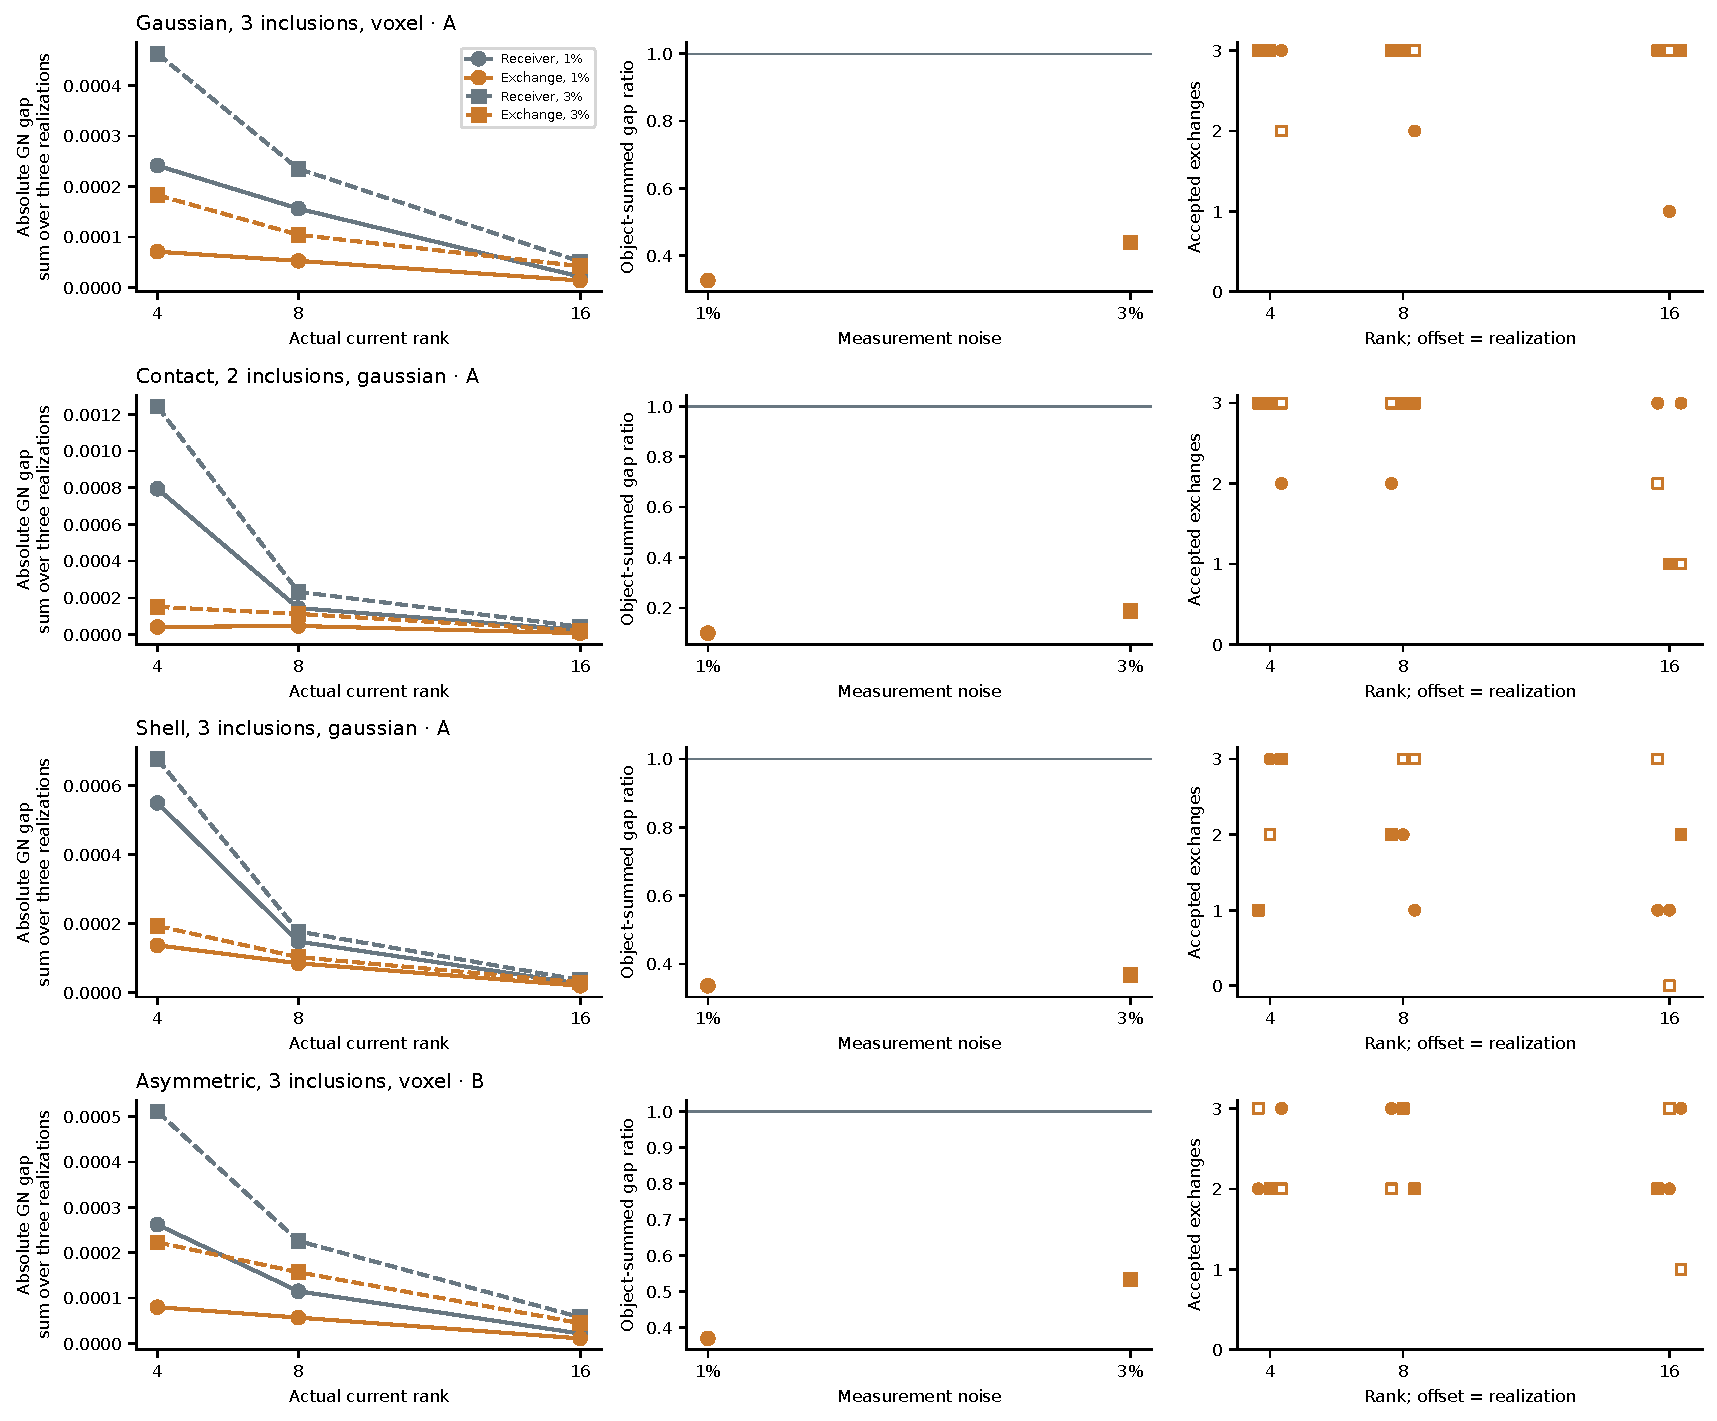
\includegraphics[width=.98\linewidth]{figures/closure_validation_v1/Figure2_noise_objects.pdf}
\caption{每行一个预选对象：左列给出三份realization的绝对gap之和，中列是对象风险比，右列是每份噪声接受了多少交换。此图没有把realization作为新的独立对象。噪声增大时某些对象收益减弱，但全部对象汇总比值仍小于1。}
\end{figure}

模式本身没有保持不变。根据保存的物理基底计算主角度（principal angles，用于衡量两个物理子空间的偏离），70/72终态相对干净情况至少有一个方向偏转10°以上，65/72达到80°以上。这是部分方向的变化，不是整个空间都被替换。材料用途依赖残差，变化可以是合理响应；所以这里报告的是收益稳定出现，而不是宣称方向选择具有不变性。

408个finalist中98个被数值复核拒绝，共接受172次交换。Jd使用2448个电流方程右端（current right-hand sides, RHS），算入Jx初始化后为2880。完整噪声作业占用895.250s；scoring、传输和Jd等嵌套阶段已包括其中。这个结果只涵盖四对象、中期、两级噪声与三份realization，不足以宣称普遍统计鲁棒性。

\section{候选覆盖：评分准确仍可能错过好方向}
假设我们知道怎样给替换打分，但只看12个移入方向。如果最有用的方向在第13个之外，再好的打分公式也选不到它。为检验这一点，离线teacher枚举固定154方向字典中的整个初次交换邻域（initial exchange neighborhood）：保留$k$列时，共有$k(154-k)$个一换一组合。无效端点照样记录；完整收益标注在部署完成之后获取，不进入selector。

令每个单元的全字典最大正收益为$Q_*^+=\max(0,\max Q)$。对象内先对这些机会求和，再用anchor选中且通过方向复核的收益之和除以它，得到排序机会捕获率（ranking opportunity capture）。十个完整额外对象为97.30--99.99\%，中位99.54\%。同样计算12候选池内最好收益可覆盖的机会，得到候选覆盖率（candidate opportunity coverage）：49.12--95.31\%，中位72.95\%。零机会不提供权重；未完成对象只有六单元的观察值，不能填成九单元总体。

\begin{figure}[htbp]\centering
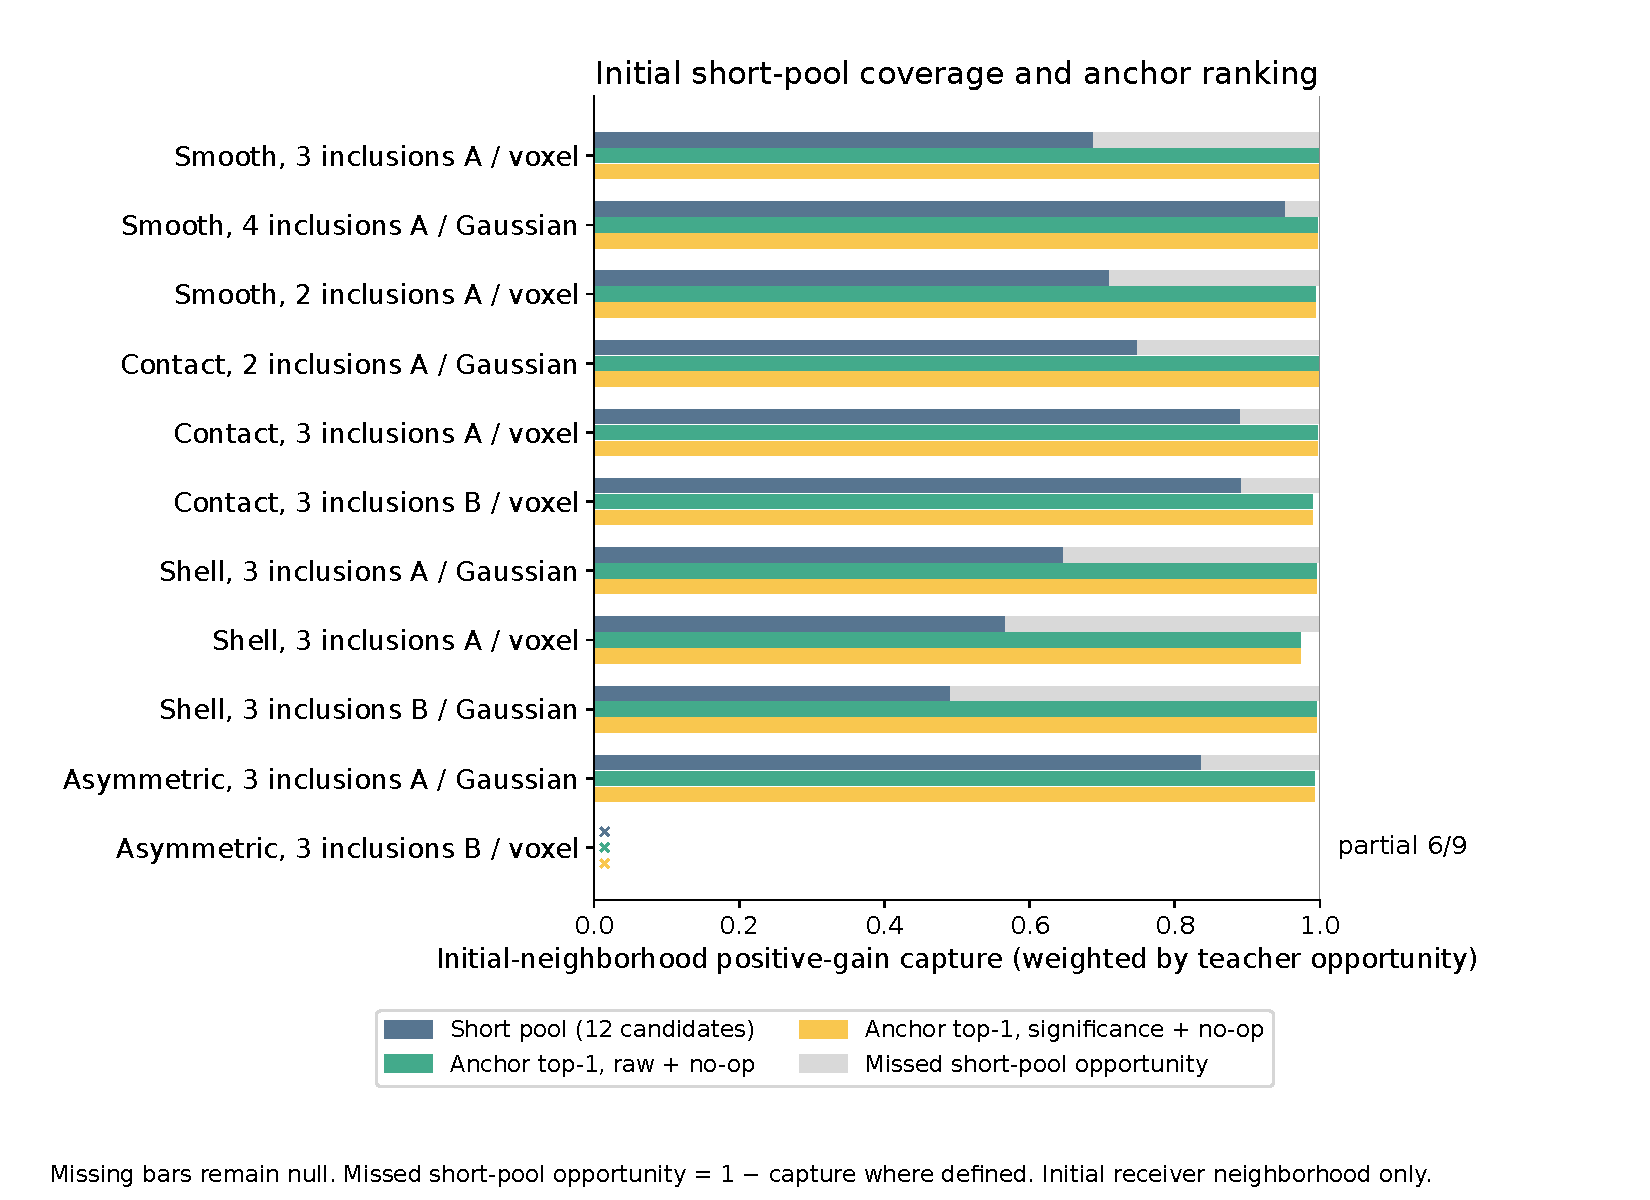
\includegraphics[width=.95\linewidth]{figures/coverage_closure_v2/initial_opportunity.pdf}
\caption{完整字典排序与固定短池覆盖是两个问题。图以对象内正收益求和后的比例呈现，非对称voxel对象的6/9观察结果单独标注。它不是最终重建误差，也不是部署整条路径的收益比例。}
\end{figure}

进一步的离线诊断最多走三个完整收益贪心动作，每次重新枚举当前邻域。它在90个单元得到更低终态gap；线上路径在5个单元更低；1个在评价底噪内相同。即使每一步都看整个字典，局部贪心也不保证全局最好，所以不能把所有终态差距称为“评分误差”。这里应分开三个问题：方向有没有送进来、送来的方向有没有排对、接受以后进入了哪个新邻域。改善候选取得是后续方向，当前冻结规则没有新增网络或再调短池。


\subsection{真正重建：为什么必须再检验一次}
冻结状态的GN比较把当前材料、总场和残差暂时固定。真正的非线性反演（nonlinear reconstruction）执行一步以后，这些量都会改变。还必须满足材料可行域（material feasibility constraints），并用线搜索（line search）判断新材料是否使完整非线性目标下降。因此，局部GN gap和最终材料误差（final material error）是两个不同指标。

固定的四个代表对象使用$k=8$，两种策略共享初始化$0.1+0.04i$、prior、LM schedule、实部下界$-0.5$、虚部下界0以及Armijo充分下降检验（Armijo acceptance）。每次先投影可行材料步，再从$\alpha=1$开始减半，最多24次；两条轨迹只改变切向电流空间。三组对照完成18次更新。

\begin{table}[htbp]\centering\small
\caption{完整三维材料相对误差：receiver $\to$ exchange。不是中心切片误差。}
\begin{tabular}{lrrr}\toprule
几何 / 表示&复材料&实部&虚部\\\midrule
平滑 / voxel&$0.3027\to0.2699$&$0.2811\to0.2516$&$0.7439\to0.6506$\\
近接触 / Gaussian&$0.6722\to0.6707$&$0.6810\to0.6835$&$0.4439\to0.2859$\\
shell / Gaussian&$0.6096\to0.5660$&$0.6081\to0.5651$&$0.6976\to0.6219$\\\bottomrule
\end{tabular}
\end{table}

三组复材料误差下降约10.8\%、0.22\%、7.16\%，留出测量误差（held-out data error）也下降。近接触对象尤其说明，数据拟合改善并不自动意味着材料所有分量改善：它的实部误差略升，复误差几乎中性。非对称voxel对象的exchange轨迹完成17次接受更新以后，在第18次更新前构建的receiver初始端点未通过预定法方程残差检查，故exchange轨迹停止。独立的receiver-only基线未运行；没有把最后安全状态当作完成终点，也不能据此推断未运行基线一定失败。

完整耗时（all-in wall time）包括每条轨迹自己的物理setup、anchor/pool获取、被拒绝的检查、line search和终点评价。三组耗时比是2.68、1.74、1.46；额外完整切向RHS分别为708、744、744，其中包含$Jx$初始化和$Jd$复核。这个方法的意义是用额外物理作用购买局部更新保真度，现有结果没有证明加速成像。

\begin{figure}[htbp]\centering
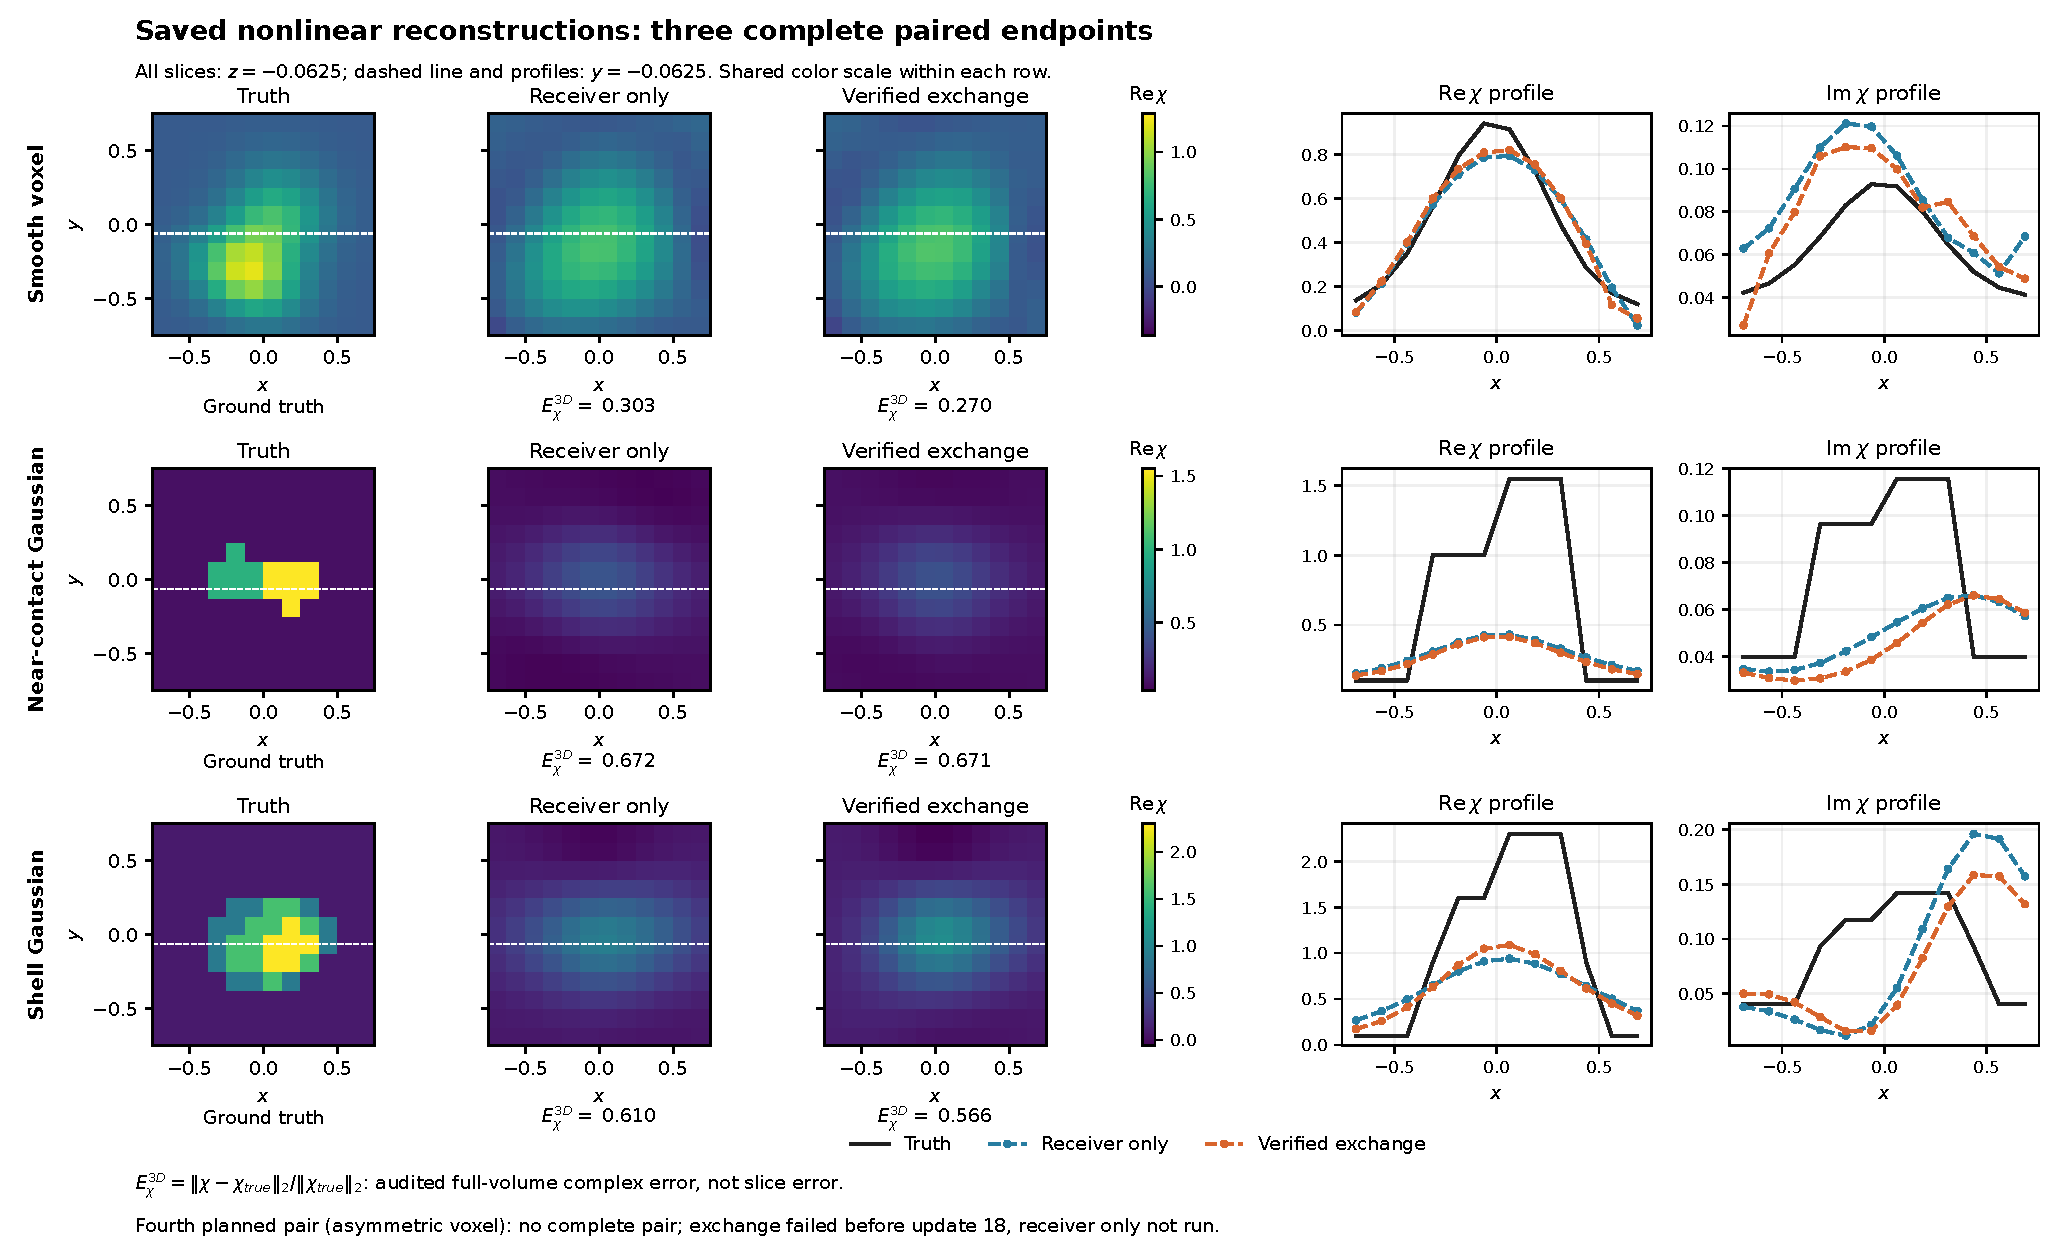
\includegraphics[width=.97\linewidth]{figures/nonlinear_closure_v1/nonlinear_reconstructions.pdf}
\caption{从左到右先看真实材料、receiver与exchange的同一中心切片，再看实部和虚部剖面线。每行统一色标，避免颜色范围不同制造视觉优势。整个体积上的误差见上表；切片仅帮助理解改善出现在哪里。接触与shell峰值仍被平滑，说明有限测量和材料表示仍限制恢复。}
\end{figure}

\begin{figure}[htbp]\centering
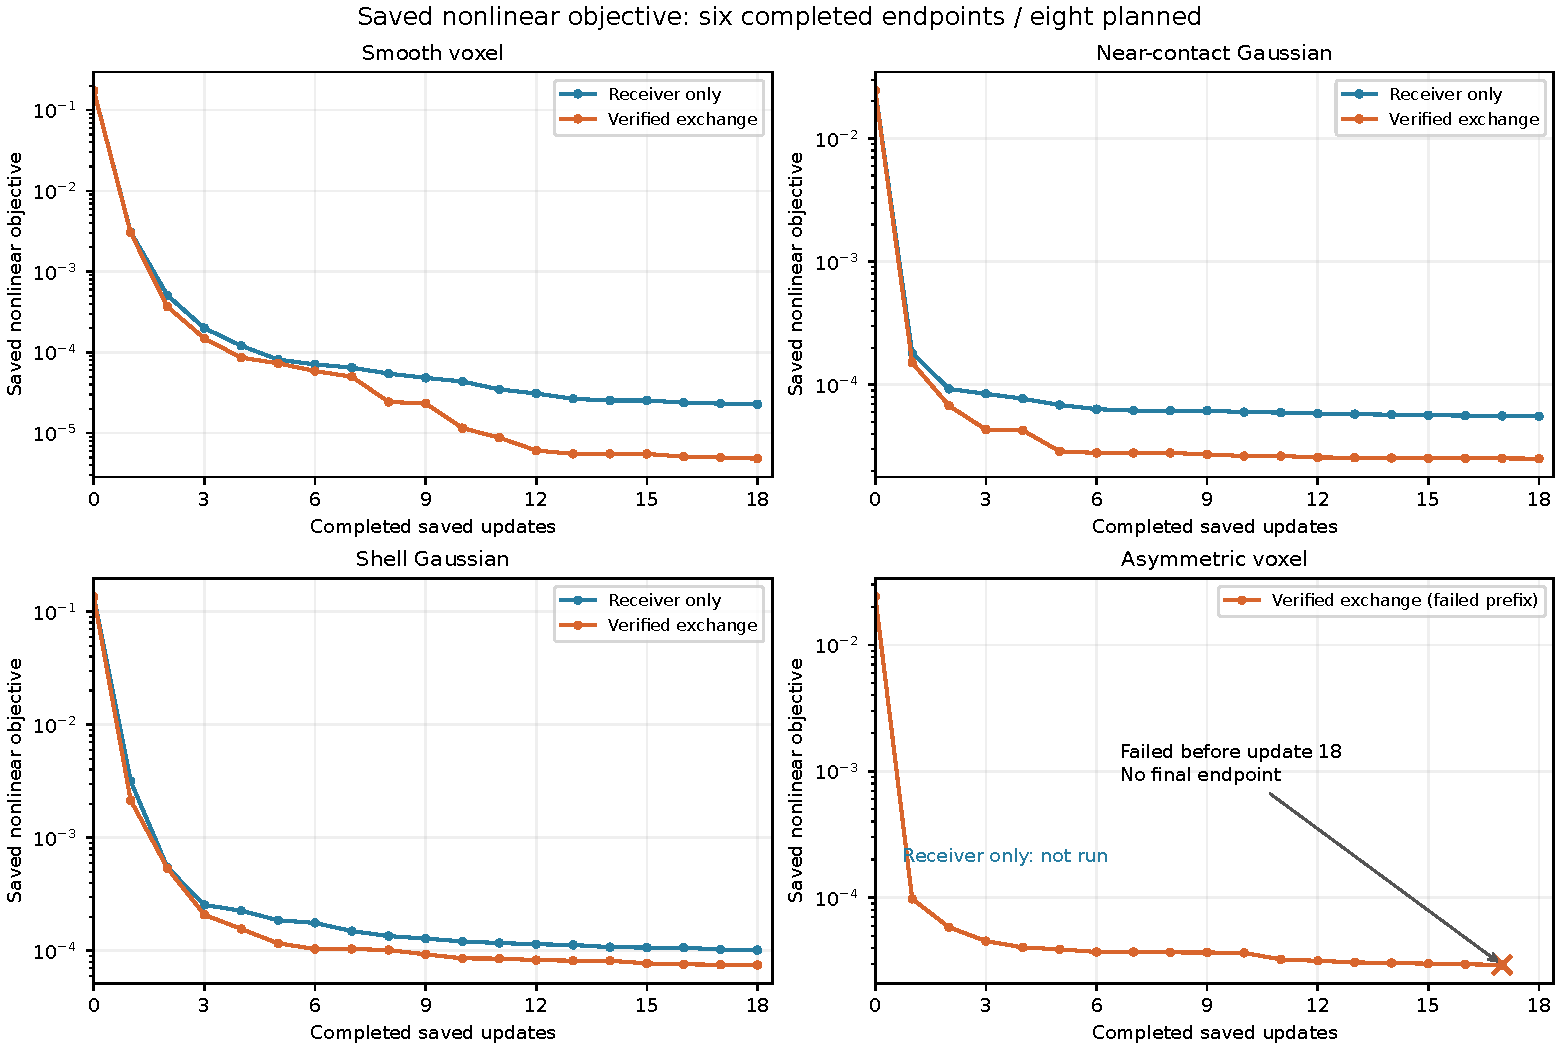
\includegraphics[width=.95\linewidth]{figures/nonlinear_closure_v1/nonlinear_objective_curves.pdf}
\caption{完整非线性目标（full nonlinear objective）随实际接受更新的变化。三个完整对照达到共同的18次更新上限。右下图单独保留非对称voxel的17步安全前缀，其后发生端点残差失败；没有对应的完成基线，不能把该曲线当作第四组成功。}
\end{figure}


\subsection{怎样阅读费用，而不被一个很快的局部耗时误导}
固定电流维数（fixed current dimension）只规定最后端点有多少列电流。为了选择这几列，exchange额外取得64列anchor、154方向字典，并支付每轮的完整方向核验（directional verification）。这些辅助信息并没有变成端点的额外列，但都需要计算和内存。被拒的候选同样已花费物理作用。

费用账本只把互不重叠的区间相加：原历史费用4889.515秒、61个闭合作业的15072.343秒，以及未进入作业的0.202秒检查，共19962.060秒，即5.545小时。子阶段、GPU上传和矩阵标签都是其中的细目，不应再加一遍。这个总数是研究执行成本，不是每个读者复现一次选择都需要的时间。

真正独立初始化的三对重建则能直接比较：receiver到exchange分别为216.46到579.89秒、407.71到710.49秒、405.90到592.29秒。三个比值都大于1。壳体所需完整forward RHS减少，总时间仍增加，说明一个环节省工作不等于整条流程加速。当前方法的工程作用是用额外计算得到更好的局部材料步，不是免费提高成像质量。



\clearpage
\section{论文解决了什么，又留下什么}
理论价值在于把指定电流改动的材料入口、内部反馈和接收返回分开，再把这些因子连接到残差相关的实际步差。已知Schur补和二次收益公式是工具；真正值得解释的是Maxwell电流怎样改变材料法方程，以及为什么可见性、信息体积和当前收益是不同判断。

实验价值在于几类证据互相约束：暗电流显示直接输出会漏掉反馈；信息正而收益负显示曲率汇总不够；pair见证显示当前相关性可能非加性；共同候选诊断显示真实有限位移的代价会改变排序。冻结规则验证则检验这种具体交换设计能否从原四对象移到更多对象，噪声和受约束重建检验其适用层次。

工程价值是把判断限制在少量可收费动作上。相同电流秩不是相同时间；缓存$Jx$和逐finalist计算$Jd$避免了多余完整伴随，但候选与anchor仍需成本。一个没有找到好动作的短池，不代表整个字典没有好方向；一个改善完整GN步的交换，也不保证最终真值误差变小。

对后续研究，最清楚的难点是候选取得（candidate acquisition）：怎样不用完整teacher就较低成本地把有价值的方向放进候选池。本文保留冻结规则，不用新增网络或调参把这个难点掩盖掉。理论成立、验证的范围和失败边界共同决定这篇论文应当怎样被使用。
\clearpage{\small\setlength{\parskip}{0pt}\begin{thebibliography}{99}
\bibitem{r1} Y. Zhong and X. Chen, ``An FFT Twofold Subspace-Based Optimization Method for Solving Electromagnetic Inverse Scattering Problems,'' \emph{IEEE Trans. Antennas Propag.}, vol. 59, no. 3, pp. 914--927, 2011, doi: 10.1109/TAP.2010.2103027.
\bibitem{r2} X. Ye and X. Chen, ``Subspace-Based Distorted-Born Iterative Method for Solving Inverse Scattering Problems,'' \emph{IEEE Trans. Antennas Propag.}, vol. 65, no. 12, pp. 7224--7232, 2017, doi: 10.1109/TAP.2017.2766658.
\bibitem{r3} X. Chen, \emph{Computational Methods for Electromagnetic Inverse Scattering}. Wiley--IEEE Press, 2018, Secs. 6.3.1 and 6.4.2.
\bibitem{r4} E. de Sturler, S. Gugercin, M. Kilmer, S. Chaturantabut, C. Beattie, and M. O'Connell, ``Nonlinear Parametric Inversion Using Interpolatory Model Reduction,'' \emph{SIAM J. Sci. Comput.}, vol. 37, no. 3, pp. B495--B517, 2015, doi: 10.1137/130946320. Author preprint: arXiv:1311.0922.
\bibitem{r5} M. Kartmann, T. Keil, M. Ohlberger, S. Volkwein, and B. Kaltenbacher, ``Adaptive Reduced Basis Trust Region Methods for Parameter Identification Problems,'' 2024, doi: 10.1007/s44207-024-00002-z. Author full text: arXiv:2309.07627v3.
\bibitem{r6} T. Bui-Thanh, K. Willcox, O. Ghattas, and B. van Bloemen Waanders, ``Goal-Oriented, Model-Constrained Optimization for Reduction of Large-Scale Systems,'' \emph{J. Comput. Phys.}, vol. 224, no. 2, pp. 880--896, 2007, doi: 10.1016/j.jcp.2006.10.026.
\bibitem{r8} A. Gaul, M. H. Gutknecht, J. Liesen, and R. Nabben, ``A Framework for Deflated and Augmented Krylov Subspace Methods,'' \emph{SIAM J. Matrix Anal. Appl.}, vol. 34, no. 2, pp. 495--518, 2013, doi: 10.1137/110820713.
\bibitem{r11} B. T. Draine and P. J. Flatau, ``Discrete-Dipole Approximation for Scattering Calculations,'' \emph{J. Opt. Soc. Am. A}, vol. 11, no. 4, pp. 1491--1499, 1994. Publisher record.
\bibitem{r16} X. Chen, Y. Zhong, and K. Agarwal, ``Subspace Methods for Solving Electromagnetic Inverse Scattering Problems,'' \emph{Methods and Applications of Analysis}, vol. 17, no. 4, pp. 407--432, 2010.
\bibitem{r17} Y. Zhong and X. Chen, ``Twofold Subspace-Based Optimization Method for Solving Inverse Scattering Problems,'' \emph{Inverse Problems}, vol. 25, art. 085003, 2009, doi: 10.1088/0266-5611/25/8/085003.
\bibitem{r18} X.-D. Chen, ``Subspace-Based Optimization Method for Solving Inverse-Scattering Problems,'' \emph{IEEE Trans. Geosci. Remote Sens.}, vol. 48, no. 1, pp. 42--49, 2010, doi: 10.1109/TGRS.2009.2025122.
\bibitem{r19} K. Xu, Y. Zhong, R. Song, X. Chen, and L. Ran, ``Multiplicative-Regularized FFT Twofold Subspace-Based Optimization Method for Inverse Scattering Problems,'' \emph{IEEE Trans. Geosci. Remote Sens.}, vol. 53, no. 2, pp. 841--850, 2015, doi: 10.1109/TGRS.2014.2329032.
\end{thebibliography}
}
\end{document}
